\chapter{Evaluierungskonzept}
\label{konzept_kon}

\section{Anwendungsbeispiel}
\label{sec:anwendung_kon}

Das Anwendungsbeispiel ist ein Kinderspiel. Dieses Spiel soll die motorischen Fähigkeiten bei Kindern verbessern.
Gegeben ist eine Kugel mit Löschern aus verschiedenen Formen(Kreis, Oval, Viereck, Trapez etc.). Zu diesen Formen existieren die  Klötzchen, die entsprechend groß sind und die Form der Löcher besitzen. Die Aufgabe des Spiel ist, alle Klötzchen in die entsprechende Form zu drücken, bis alle in der Kugel sind.

\begin{figure}[H]
  \centering
    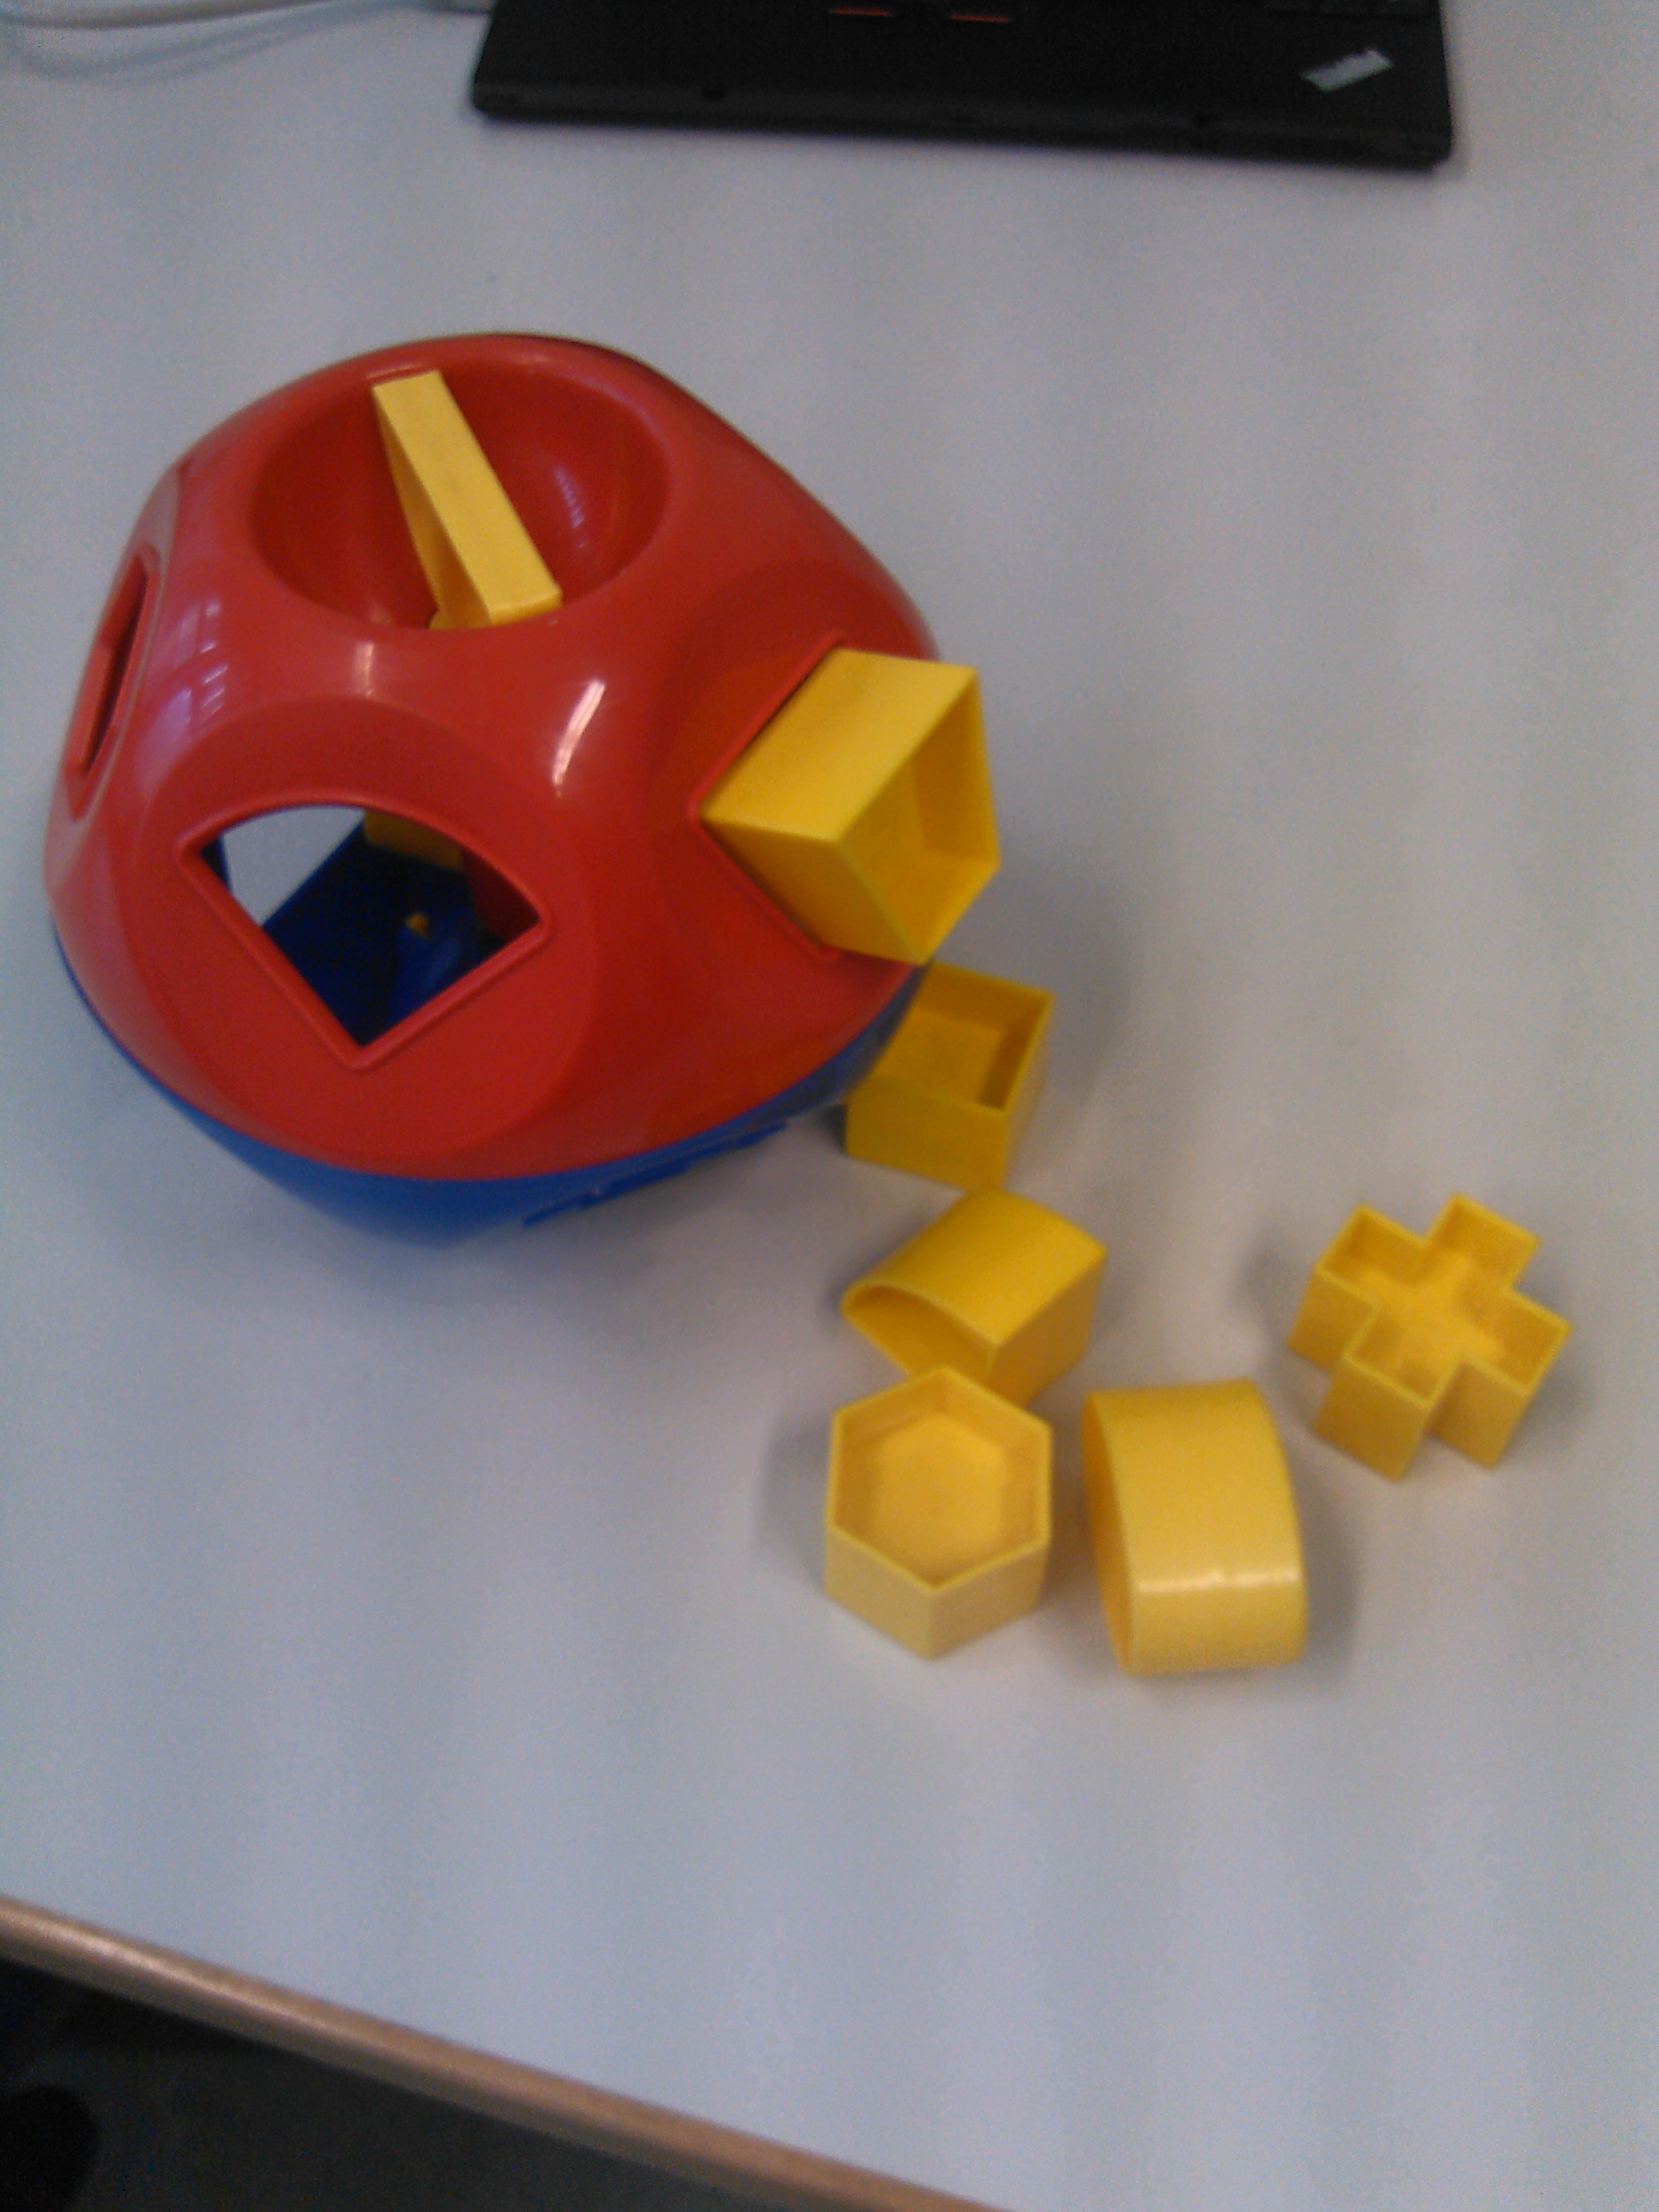
\includegraphics[width=0.5\textwidth]{pic/spiel.jpg}
      \caption[Kinder Geschicklichkeitsspiel]{Kinderspiel zur Evaluierung der Software Schnittstellen}
      \label{fig:kinderspiel}
\end{figure}
\newpage

Die Kugel wird am Kopf des Roboterarms befestigt. Es soll eine Anwendung entwickelt werden, die für einen Spieler die Höhe des Roboters einstellt. Der Spieler soll die Möglichkeit haben, die Startposition zu verstellen und für sich zu speichern. Bei einem bestimmten Knopfdruck soll der Roboter das Loch für die jeweils nächste Form so ausrichten, damit der Mensch das Klötzchen nur noch einzuwerfen braucht.

\section{Speichern der Anwendungsdaten}
\label{sec:save_of_data_kon}

Um auf bestimmte Menschen zugeschnittene Bewegungen ablaufen zu lassen, muss der Roboter Daten über den Anwender kennen. Diese sollten persistent gespeichert werden, damit bei einem Wechsel des Anwenders die Daten nicht verloren gehen.
Daten der Anwender sind z.B. Name, Alter, bestimmte Positionen im Roboter-Programm, etc.
\\\\
\textbf{Speichern über Polyscope und URScript}
\label{sec:save_data_polyscope_kon}
\\\\
In der Polyscope Software oder in einem URScript Programm können Daten, die von den Benutzern erstellt oder erhoben werden, nicht persistent
gespeichert werden. Hierzu muss eine zweite Anwendung entwickelt werden, auf die sich das URScript oder \ac{URP} verbindet und die Daten zum persistenten Speichern versendet.
In Polyscope und URScript muss sehr aufwendig mit den vorhandenen Skriptbefehlen eine Socket\footnote{Ein Socket ermöglicht ein Datenaustausch zwischen Programmen im Rechner oder auch zwischen zwei verschiedenen Host-Systemen} Verbindung aufgebaut werden.
Damit diese zwei Programme miteinander kommunizieren können, muss ein gemeinsames Protokoll mit bestimmten Befehlen festgelegt werden. Es ist möglich Text, Ganzzahlen oder Dezimalzahlen zu versenden und zu empfangen. Es kann nur einer dieser drei Typen versendet werden, von diesem aber beliebig viel.
\\\\
\textbf{Speichern über Eigene API}
\label{save_data_own_api_kon}
\\\\
Mit der eigenen API muss keine zweite Software entwickelt werden, da die API auf einem Client Rechner läuft und dort die Daten persistent gespeichert werden können. Es muss jedoch im Anwendungsprogramm eine Verbindung zu einer Datenbank aufgebaut werden, um dort die Daten speichern zu können.